\documentclass[11pt]{article}

\usepackage{parskip}
\usepackage{graphicx}
\usepackage{amsmath}
\usepackage{listings}

\usepackage[T1]{fontenc}
\usepackage{lmodern}

\usepackage{pythonhighlight}

% Margins
\topmargin=-0.45in
\evensidemargin=0in
\oddsidemargin=0in
\textwidth=6.5in
\textheight=9.0in
\headsep=0.25in

\title{605.744: Information Retrieval \\ Programming Assignment \#1: Corpus Statistics}
\author{Sabbir Ahmed}
\date{\today}

\begin{document}
\maketitle	

\section{Introduction}
This paper describes a collection of scripts written to compute the term-frequency, document-frequency, and other statistics from a pre-generated corpus.

\section{Technical Background}
All of the source code is in Python 3.10. The program is split into several modules and follows an object oriented structure. The following is the directory structure of the source code:

\begin{figure}[!ht]
    \caption{Directory Hierarchy of Assignment 1}
    \centering
    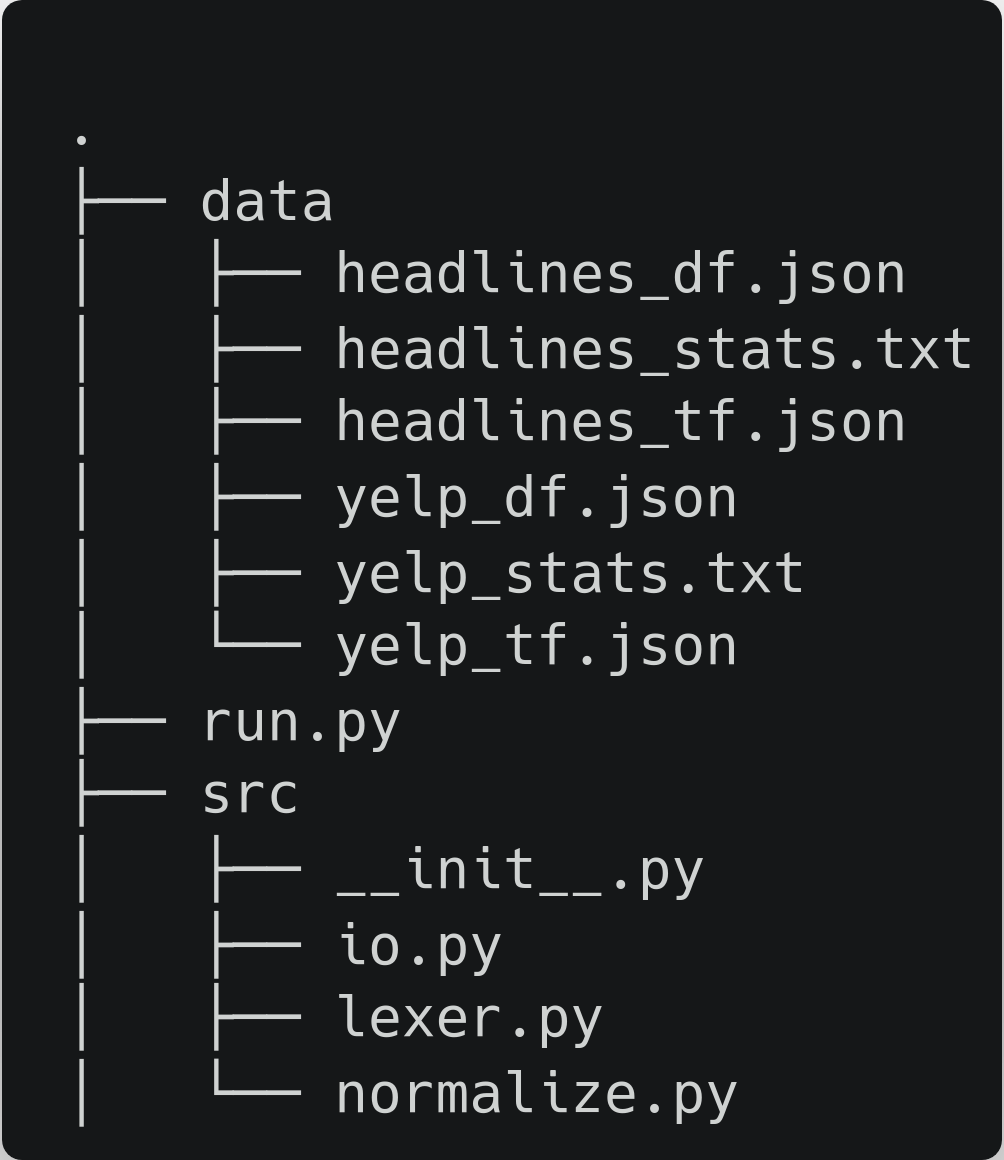
\includegraphics[scale=0.2]{statics/dirtree.png}
\end{figure}

The source code for all of the files are attached in Appendix \ref{appendix:src}.

The total number of non-empty lines of code for the program comes to 200, with an average execution time of 40 seconds to process both of the sample files.

\begin{figure}[!ht]
    \caption{UML of Corpus Statistics}
    \centering
    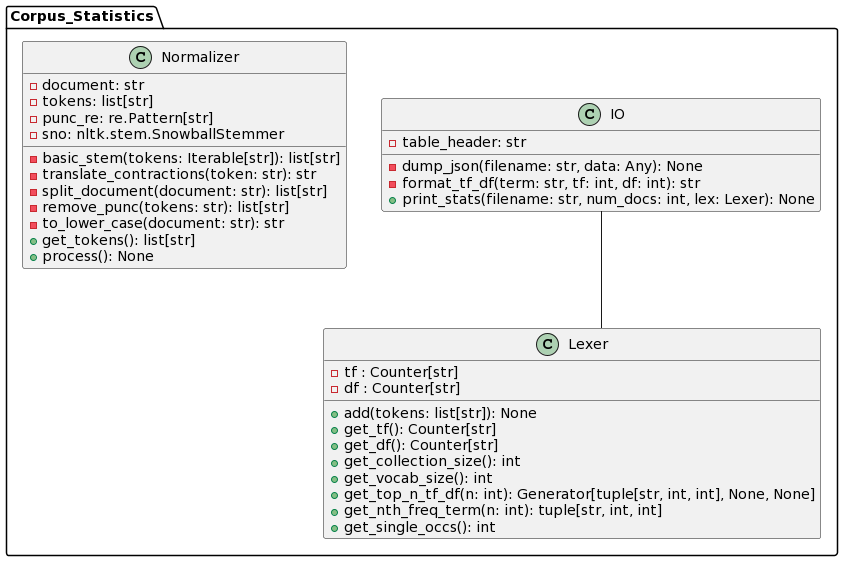
\includegraphics[scale=0.6]{statics/uml.png}
\end{figure}

\subsection{Driver} \label{sec:driver}
The driver script for the program is \texttt{run.py}. The file is responsible for opening up the input files, reading in all of the documents contained in those files, processing them into the lexicon, and generating and saving statistics on them. Since the sample files are relatively small, the entire content may be loaded into the memory of a modern machine. However, to account for possible larger files, the lines containing the documents are saved in memory, normalized, and added to the lexicon before moving to the next document.

This method of reading the files imposes a limitation, where every document is assumed to be on the 2nd line out of 4 (line\_num \% 4 == 1). The algorithm will need to be modified if the files in the future have different formats.

\subsection{\texttt{normalize.Normalizer}}
The \texttt{Normalizer} class normalizes the documents. The class is instantiated once and it provides a method to set the document for normalization. The normalization pipeline includes the following processes, in order:

\begin{enumerate}
    \item translating the entire document to lower case. The document is unconditionally transformed into lower case, which can lead to confusion with words that are considered proper nouns.

    \item splitting the document on whitespace into tokens.

    \item expanding word contractions into their components. The contractions are pre-generated into a Python dict in \texttt{normalize.CONTRACTIONS} for constant-time look-ups.

    \item splitting the tokens on all punctuations except "'". The "'" is preserved for the stemmer to process later. Not splitting on this character also avoids including incorrect tokens into the lexicon. For example, "food's" will get tokenized into ["food", "s"].

    \item rejoining and splitting the tokens to remove empty tokens.

    \item stemming tokens with nltk.stem.SnowballStemmer.stem(word).
\end{enumerate}

The tokens are available as a list of string to be added into the lexicon before being overwritten by the next document.

\subsubsection{External Libraries}
The external library \texttt{nltk} was used for its stemming capabilities. The stemmers \texttt{PorterStemmer} and \texttt{SnowballStemmer} were tested over a sample of the documents, and the latter algorithm appeared to yield subjectively better-looking results.

\subsection{\texttt{lexer.Lexer}}
The \texttt{Lexer} class utilizes 2 \texttt{collections.Counter} objects to store the term-frequency and document-frequency of the lexicon. The bag-type container is a part of the standard library and match in performance compared to default \texttt{dict}s, but with additional methods such as \texttt{Counter.total()}, \texttt{Counter.most\_common(n)}, etc. These methods are helpful in generating statistics required in the assignment.

\section{Statistics and Observations}
Since stopwords were not removed, they were prominent in the 100 most frequent terms in both of the files. "the" and "to" were present in the top 5 most frequent terms in both of the sets of documents. In the Yelp corpus, some of the most commonly occurring words were related to food and restaurant services. This theme is expected due to the source of the documents containing reviews of mostly food service establishments and its quality. The Headlines corpus did not appear to circulate a theme, although some of the frequent words appeared to be numerical or date values. This can be expected due to the source of the documents mostly discussing events with timelines. The numerical values can indicate money, percentage, weather, length of service, etc.

Both of the corpora had an almost identical percentage of singly-occurring terms (~48.8\%). These are terms that appeared in only one document.

\appendix

\section{Source Code} \label{appendix:src}

\inputpython{./src/io.py}{./src/io.py}
\inputpython{./src/normalize.py}{./src/normalize.py}
\inputpython{./src/lexer.py}{./src/lexer.py}

\inputpython{./run.py}{./run.py}

\end{document}
